%DOCUMENT
\documentclass[11pt,reqno]{amsart}
\usepackage[margin=1.23in, footskip=.4in]{geometry}
%FONT
\usepackage[T1]{fontenc}
\usepackage[american]{babel}
%PACKAGES
\usepackage{amsmath,amsfonts,amssymb,amsthm,wasysym,bm}
\usepackage{mathrsfs}
\usepackage{hyperref}
\usepackage{graphicx}
\usepackage[justification=centering]{caption}
\usepackage{subcaption}
\usepackage{multicol}
\usepackage[table,xcdraw]{xcolor}
%package for pictures
\usepackage{float}
\usepackage{enumitem}
\usepackage[europeanresistors, cuteinductors]{circuitikz} 
%THEOREMS
\newtheorem{theorem}{Theorem}[section]
\newtheorem*{theorem*}{Theorem}
\newtheorem{proposition}[theorem]{Proposition}
\newtheorem{corollary}[theorem]{Corollary}
\newtheorem{lemma}[theorem]{Lemma}
\newtheorem*{conjecture*}{Conjecture}
\theoremstyle{definition}
\newtheorem{definition}{Definition}[section]
\newtheorem{remark}{Remark}[section]
\newtheorem{assumption}{Assumption}
\newtheorem*{notation}{Notation}
\numberwithin{equation}{section}
\theoremstyle{remark}
\newtheorem{example}{Example}[section]
\newcommand{\mbbR}{{\mathbb R}}
\newcommand{\mbbN}{{\mathbb N}}
\def\mcA{\mathcal{A}}
\def\mcC{\mathcal{C}}
\newcommand{\E}{\mathcal{E}}
\newcommand{\F}{\mathcal{F}}
\newcommand{\D}{\mathcal{D}}
\def\mcH{\mathcal{H}}
\def\mcR{\mathcal{R}}
\def\mcS{\mathcal{S}}
\def\mcT{\mathcal{T}}

\newcommand{\SG}{\operatorname{SG}}
\newcommand{\I}{\operatorname{I}}
\newcommand{\diam}{\operatorname{diam}}
\newcommand{\supp}{\operatorname{supp}}
\newcommand{\dom}{\operatorname{dom}}

\newcommand{\rH}{r_{\text{H}}}
\newcommand{\rI}{r_{\I}}
\newcommand{\rSG}{r_{\SG}}

\def\ss#1{\scriptscriptstyle{#1}}
\def\sss#1{\scriptscriptstyle{(#1)}}
\def\rh#1#2{\rho^{\scriptscriptstyle{(#1})}_{#2}}
\def\gam#1#2{\gamma^{\scriptscriptstyle{(#1})}_{#2}}
\providecommand{\V}[2]{V_{#1}^{#2}}
\providecommand{\ask}[1]{\textcolor{magenta}{#1}}
\DeclareMathOperator*{\argmax}{arg\,max}
\DeclareMathOperator*{\argmin}{arg\,min}
%page style
\setlength{\parindent}{0pt}

%%%%%%%%%%%%%%%%%%%%%%%%%%%%%%%%%%%%%%%%%%%%%%%%%%%

\begin{document}
\title[Robust Control of Markov Decision Process]{Robust Control of Markov Decision Processes: Literature Review and Applications}
\author[A. Biswas \and Z. Cao \and H. Gu \and J. Ye \and S. Zhu]{Ayan Biswas \and Zhe Cao \and Haotian Gu \and Jiayu Ye \and Shizhan Zhu\\UC Berkeley}
\maketitle
\vspace{-15pt}
\begin{abstract}
% This is a course project report for EE227B: Convex Optimization. In this project, we do a literature review of robust control of Markov Decision Processes (MDP), specifically focusing on:
% \begin{enumerate}
% \item Formulating the robust MDP under different scenarios
% \item Analyzing the tractability of the robust counterpart
% \item Solving the robust counterpart using theories such as duality, support functions
% \item Exploring the real-world applications and comparing the performance of the robust counterpart with the nominal problem 

% \end{enumerate}
Markov Decision problems are encountered frequently in real-life applications. The problems are often prone to uncertainties in environment dynamics. In many practical problems, ignorance of potential risk limits the performance of the optimal policy. This is a well explored field with lots of rich literature. We reviewed some relevant papers and summarized the different formulations of the Markov Decision Process, specifically focusing on uncertainty pertaining to two settings: uncertainty in reward/cost and uncertainty in transition dynamics. We conducted two numerical experiments to verify the efficacy of uncertainty set modelling. The first experiment is the classic aircraft path routing problem when the storm map in the environment follows an uncertain Markov Process. The other is the machine replacement problem, with uncertain replacement cost and uncertain transition matrix. Our experimental results showed the general improvement of the optimized performance when uncertainty sets are modelled with robust or chance-constraint formulations. 
\end{abstract}

%\newpage
%\tableofcontents
%\newpage
\vspace{20pt}

%%%%%%%%%%%%%%%%%%%%%%%%%%%%%%%%%%%%%%%%%%%%%%%%%%%
\section{Overview}
The report is organized as follows. In Sec. 2, we introduce the theory of Markov Decision processes with finite and infinite time horizons.
Sec. 3 presents the general problem formulation of Markov Decision Processes with uncertain costs, while Sec. 4 elaborates the uncertain transition parameters case. In Sec. 5, we dive into the first application of Aircraft Routing Problem, while in Sec. 6 we present the experimental results for the Machine Replacement problem. Finally we conclude the paper in Sec. 7.

%\newpage
\medskip

\section{Markov Decision Processes}

%%%%%%%%%%%%%%%%%%%%%%%%%%%%%%%%%%%%%%%%%%%%%%%%%%%

\subsection{Problem Formulation}
A Markov Decision Process $M = (\mathcal{S}, \mathcal{A}, T, P, C, \gamma)$ consists of the following components: 
\begin{itemize}
    \item a finite state space $\mathcal{S}$
    \item a finite action space $\mathcal{A}$
    \item a finite or infinite time horizon $T$
    \item a collection of transition matrices $\{P^a_t\}_{a\in\mathcal{A},t=0\ldots T-1}$ where $P^a_t(i,j)$ is the probability of transiting from state $i$ to $j$ when playing action $a$ at time $t$
    \item a collection of cost functions $\{C_t\}_{t=0\ldots T}$ where $C_t(i, a)$ corresponds to a cost the player needs to pay when playing action $a$ at state $i$ at time $t$, and $C_T(i)$ corresponds to a terminal cost
    \item a discount factor $\gamma$ when $T$ is infinite
\end{itemize}
We use $q$ to denote a distribution on $A$ which is satisfied by the initial state $i_0$.

\medskip

 A policy $\pi=(\pi_0\ldots\pi_{T-1})\in\Pi$ can be viewed as a function that specifies the action that the player will choose when in state $s$ at time $t$. The goal is to find $\pi$ to minimize the cost over $T$. There are several types of policies studied in this report. 
 \begin{itemize}
     \item A policy is called deterministic if each $\pi_t$ is a mapping from $\mathcal{S}$ to $\mathcal{A}$. We denote the set of deterministic policies by $\Pi_d$.
     \item A policy is called stochastic if each $\pi_t$ is a mapping from $\mathcal{S}$ to a probability distribution on $\mathcal{A}$. We denote the set of stochastic policies by $\Pi_s$.
     \item A policy is called stationary if $\pi_t$ is invariant over time $t$.  We use $\Pi^s$ to denote the set of stationary policies.
 \end{itemize}

\medskip

When $T$ is finite, given $M = (\mathcal{S}, \mathcal{A}, T, P, C)$, the nominal MDP is to find
\begin{equation}\label{nominal-mdp-finite}
    \phi_T(\Pi,P):=\min_{\pi\in\Pi}C_T(\pi,P):=\min_{\pi\in\Pi}\mathbb{E}_{\pi,P} \left[\sum_{t=0}^{T-1} C_t(i_t, \pi_t(i_t))+C_T(i_T)\right].
\end{equation}
When T is infinite, we often consider the stationary cost functions and transition matrices, which means $C_t=C,P^a_t=P^a$ for any $t$. In this case, we restrict ourselves to consider the stationary policies. So the nominal problem is
\begin{equation}\label{nominal-mdp-infinite}
    \phi_\infty(\Pi^s,P):=\min_{\pi\in\Pi^s}C_\infty(\pi,P):=\min_{\pi\in\Pi^s}\mathbb{E}_{\pi,P} \left[\sum_{t=0}^{\infty}\gamma^t C(i_t, \pi(i_t))\right].
\end{equation}

%%%%%%%%%%%%%%%%%%%%%%%%%%%%%%%%%%%%%%%%%%%%%%%%%%%

\subsection{Markov Decision Processes with Finite Time Horizon}

%%%%%%%%%%%%%%%%%%%%%%%%%%%%%%%%%%%%%%%%%%%%%%%%%%%

\subsubsection{Dynamic Programming: Policy Iteration and Value Iteration}
To get an optimal policy in $\Pi_d$ for the problem~\ref{nominal-mdp-finite}, we can apply the following dynamic programming techniques. Let $v_t(i)$ be the optimal value function at time $t$ and state $i$.
\begin{gather}\label{nominal-dynamic}
v_t(i)=\min_{a\in\mathcal{A}}\left[C_t(i,a)+\sum_{j\in\mathcal{S}}P^a_t(i,j)v_{t+1}(j)\right]\\
\pi_t(i)=\argmin_{a\in\mathcal{A}}\left[C_t(i,a)+\sum_{j\in\mathcal{S}}P^a_t(i,j)v_{t+1}(j)\right]
\end{gather}

%%%%%%%%%%%%%%%%%%%%%%%%%%%%%%%%%%%%%%%%%%%%%%%%%%%

\subsubsection{Linear Programming Formulation}
\ref{nominal-mdp-finite} can also be formulated as a LP and the detailed discussion can be found in~\cite{puterman2014markov}.
\begin{equation}\label{lp:finite}
    \begin{gathered}
    \max_{v_0\ldots v_{N-1}} \; \sum_{i\in\mathcal{S}}q(i)v_0(i) \\
    \text{s.t.} \; v_t(i)\leq C_t(i,a)+\sum_{j\in\mathcal{S}}P_t(j|i,a)v_{t+1}(j)\quad\forall a\in\mathcal{A},i\in\mathcal{S},t=0\ldots T-1
\end{gathered}
\end{equation}

\newpage
%%%%%%%%%%%%%%%%%%%%%%%%%%%%%%%%%%%%%%%%%%%%%%%%%%%

\subsection{Markov Decision Processes with Infinite Time Horizon}

%%%%%%%%%%%%%%%%%%%%%%%%%%%%%%%%%%%%%%%%%%%%%%%%%%%

\subsubsection{Bellman Recursion: Policy Iteration and Value Iteration}
Let $v(i)$ be the optimal value function at state $i$. Then the optimality condition is 
\begin{equation}\label{bellman-optimal-condition}
    v(i)=\min_{a\in\mathcal{A}}\left[C(i,a)+\gamma\sum_{j\in\mathcal{S}}P^a(i,j)v(j)\right].
\end{equation}
Define the Bellman operator $T$ on $\mathbb{R}^{|\mathcal{S}|}$, such that for any $u\in\mathbb{R}^{|\mathcal{S}|}$,
\begin{equation}
    Tu(i)=\min_{a\in\mathcal{A}}\left[C(i,a)+\gamma\sum_{j\in\mathcal{S}}P^a(i,j)u(j)\right].
\end{equation}
 The optimal value function $v$ is the unique fixed point of $T$ and it can be obtained by fixed point iterations. Furthermore, an optimal policy can be obtained by
 \begin{equation}
    \pi(i)=\argmin_{a\in\mathcal{A}}\left[C(i,a)+\gamma\sum_{j\in\mathcal{S}}P^a(i,j)v(j)\right].
\end{equation}

%%%%%%%%%%%%%%%%%%%%%%%%%%%%%%%%%%%%%%%%%%%%%%%%%%%

\subsubsection{Linear Programming Formulation}
\ref{nominal-mdp-infinite} can also be formulated as a LP and the detailed discussion can be found in~\cite{puterman2014markov}.
\begin{equation}\label{lp:infinite}
    \begin{gathered}
    \max_{v} \; \sum_{i\in\mathcal{S}}q(i)v(i) \\
    \text{s.t.} \; v(i)\leq C(i,a)+\gamma\sum_{j\in\mathcal{S}}P(j|i,a)v(j)\quad\forall a\in\mathcal{A},i\in\mathcal{S}
\end{gathered}
\end{equation}


%%%%%%%%%%%%%%%%%%%%%%%%%%%%%%%%%%%%%%%%%%%%%%%%%%%

\section{Markov Decision Processes Under Uncertain Costs}
In the previous discussion, we see how the nominal MDP problem is solved by dynamic programming or linear programming. But in real-world applications, it is natural to encounter situations where costs or transition probabilities are uncertain. In this section, we will focus on solving MDP problems under uncertain costs. To simplify the discussion, we will only consider the infinite horizon MDP, but the methodologies we introduce can be easily extended to the finite horizon case. We mainly refer to~\cite{delage2010percentile} and~\cite{xu2010distributionally} for results in this section.

%%%%%%%%%%%%%%%%%%%%%%%%%%%%%%%%%%%%%%%%%%%%%%%%%%%

\subsection{Problem Formulation}
There are different ways to model the uncertainty on cost functions. For example, we can assume now the cost functions are random variables, $C\sim\mu$, where $\mu$ can either be a known distribution or an unknown distribution belonging to some class $U$. For the first case, as also mentioned in the lecture, one usual approach is to add a chance constraint to the nominal problem~\ref{nominal-mdp-infinite}:
\begin{equation}\label{cost-chance}
\begin{gathered}
    \min_{\pi\in\Pi^s, y} y \\
    \text{s.t. } \mathbb{P}_{C}\left(\mathbb{E}_{\pi,P} \left[\sum_{t=0}^{\infty}\gamma^t C(i_t, \pi(i_t))\right] \le y\right)\ge 1-\epsilon.
\end{gathered}
\end{equation}
For the second case, we can consider the distributionally robust policy
\begin{gather}\label{cost-dist-robust}
    \min_{\pi\in\Pi^s}\max_{C\sim\mu\in U}\mathbb{E}_{\pi,P} \left[\sum_{t=0}^{\infty}\gamma^t C(i_t, \pi(i_t))\right] 
\end{gather}
And this formulation is studied in~\cite{xu2010distributionally}. In the remaining part of this section, we will focus on the first case.

%%%%%%%%%%%%%%%%%%%%%%%%%%%%%%%%%%%%%%%%%%%%%%%%%%%

\subsection{Chance Constraint: Theory and Derivation}
At a first glance, solving~\ref{cost-chance} seems to be complicated. However, after dualizing~\ref{lp:infinite}, we arrive at the following LP:
\begin{equation}\label{lp:dual-infinite}
\begin{gathered}
    \min_{\rho}\sum_{i\in\mathcal{S},a\in\mathcal{A}}\rho(i,a)C(i,a) \\
    \text{s.t. } q(i)-\sum_{a\in\mathcal{A}}\rho(i,a)+\gamma\sum_{j\in\mathcal{S},a\in\mathcal{A}}P(i|j,a)\rho(j,a)=0,\\
    \rho\geq0.
\end{gathered}
\end{equation}
Note that in this form, the only uncertainty is in the objective. Hence, the chance programming~\ref{cost-chance} is equivalent to 
\begin{equation}\label{chance}
\begin{gathered}
    \min_{\rho,y}y\\
    \text{s.t. } \mathbb{P}_C\left(\sum_{i\in\mathcal{S},a\in\mathcal{A}}\rho(i,a)C(i,a)\leq y\right)\geq1-\epsilon\\
    q(i)-\sum_{a\in\mathcal{A}}\rho(i,a)+\gamma\sum_{j\in\mathcal{S},a\in\mathcal{A}}P(i|j,a)\rho(j,a)=0,\\
    \rho\geq0.
\end{gathered}
\end{equation}
In general, there are a rich theory on how to deal with the chance constraint in~\ref{chance}. For example, in the lecture, we have studied how to build the Bernstein approximation to turn the problem into a tractable form. Meanwhile, for some special classes of distributions, we can further simplify the problem. One case is presented in the next subsection.

\medskip

The other remark is that, after solving~\ref{chance} and get $\rho^*$, we still want to recover an optimal condition. In~\cite{puterman2014markov}, it has been proved that there is a 1-1 correspondence between the feasible solution $\rho$ and the policy space $\Pi^s_s$. More explicitly, we can define the optimal policy $\pi^*$ by
\begin{equation}\label{rho-to-policy}
\pi^*(i,a) = \begin{cases}
\frac{1}{|\mathcal{A}|} &\text{if $\sum_{a\in\mathcal{A}}\rho^*(i,a)$ = 0}\\
\frac{\rho^*(i,a)}{\sum_{a\in\mathcal{A}}\rho^*(i,a)} &\text{otherwise}
\end{cases}
\end{equation}

%%%%%%%%%%%%%%%%%%%%%%%%%%%%%%%%%%%%%%%%%%%%%%%%%%%

\subsection{Case Study: Cost Uncertainty with Gaussian Distribution}
Now assume $C$ satisfies the multivariate Gaussian distribution $\mathcal{N}(\mu_C,\Theta_C)$ Under this setting, it is well-known that the constraint
\begin{equation}\label{chance-constraint}
    \mathbb{P}_C\left(\sum_{i\in\mathcal{S},a\in\mathcal{A}}\rho(i,a)C(i,a)\leq y\right)\geq1-\epsilon
\end{equation}
is equivalent to
\begin{equation}\label{socp}
    \sum_{i\in\mathcal{S},a\in\mathcal{A}}\rho(i,a)\mu_C(i,a)+\Phi^{-1}(1-\epsilon)\sqrt{\rho^T\Theta_C\rho}\leq y
\end{equation}

Hence, if $C$ is Gaussian, then this problem is equivalent to an SOCP.

\medskip

One simple generalization of~\ref{chance-constraint} is that, instead of assuming $C\sim\mathcal{N}(\mu_C,\theta_C)$, we can consider the moment constraints
\begin{equation}\label{moment-constraint}
\begin{gathered}
\mathbb{P}_C\left(\sum_{i\in\mathcal{S},a\in\mathcal{A}}\rho(i,a)C(i,a)\leq y\right)\geq1-\epsilon,\\
\forall C~\text{s.t.}~\mathbb{E}[C]=\mu_C,~\mathbb{E}\left[(C-\mu_C)(C-\mu_C)^T\right]=\Theta_C
\end{gathered}
\end{equation}
It is also a well-known fact that~\ref{moment-constraint} is equivalent to
\begin{equation}\label{generalized-chebyshev}
    \sum_{i\in\mathcal{S},a\in\mathcal{A}}\rho(i,a)\mu_C(i,a)+]\sqrt{\frac{1-\epsilon}{\epsilon}}\sqrt{\rho^T\Theta_C\rho}\leq y.
\end{equation}
More detailed discussions can be found in~\cite{ben2009robust}.
%%%%%%%%%%%%%%%%%%%%%%%%%%%%%%%%%%%%%%%%%%%%%%%%%%%

\section{Markov Decision Processes Under Uncertain Transition Parameters}
In this section, we will focus on dealing with uncertain transition parameters. As before, we will still present results only for the infinite horizon MDP, and these results can be extended to the finite horizon case easily. We mainly refer to~\cite{nilim2005robust} and \cite{wiesemann2013robust}.

%%%%%%%%%%%%%%%%%%%%%%%%%%%%%%%%%%%%%%%%%%%%%%%%%%%

\subsection{Problem Formulation}There are several different approaches to model the uncertainty on transition parameters. Similar to what we have discussed in the previous section, one possible formulation is to assume transition parameters are random variables and then to introduce chance constraints on transition matrices. This problem is studied in~\cite{delage2010percentile}. But it turns out that the chance programming on $P$ is in general very difficult to deal with, even when we only consider the Dirichlet random variables. Some computationally tractable approximation approaches are proposed to handle this problem. See~\cite{delage2010percentile} for more details.

\medskip

Another possible formulation is that, for each action $a$, the corresponding transition matrix $P^a$ is only known to lie in some set of confidence $\mathcal{P}^a$. $P=\{{P^a}\}_{a\in\mathcal{A}}\in\bigotimes_{a\in\mathcal{A}}\mathcal{P}^a:=\mathcal{P}$. The robust counterpart of~\ref{nominal-mdp-infinite} is stated as
\begin{align}\label{robust-mdp}
    C^*=\min_{\pi\in\Pi^s} \max_{P\in\mathcal{P}} \mathbb{E}_{\pi, P} \left[\sum_{t=0}^{\infty}\gamma^t C(i_t, \pi(i_t))\right].
\end{align}
If $\mathcal{P}$ is a confidence region that contains the true transition parameter $P$ with probability $1-\beta$, then we want to find a policy $\pi$ that guarantees an expected total cost of at most $C^*$ at a confidence level $1-\beta$.

\medskip

In~\cite{nilim2005robust}, this problem has been studied, for both the finite horizon and the infinite horizon, under the so-called `rectangular uncertainty property'. More specifically, it means that for every $a\in\mathcal{A}$, $\mathcal{P}^a$ has the form $\mathcal{P}^a=\bigotimes_{i\in\mathcal{S}}\mathcal{P}^a_i$, where $\mathcal{P}^a_i$ is some given subset of the probability simplex in $\mathbb{R}^{|\mathcal{S}|}$ that describe the uncertainty on the state distribution given action $a$ at state $i$.

\medskip

In remaining part of this section, we will first follow the framework of~\cite{nilim2005robust} and see how~\ref{robust-mdp} is solved by the robust version of Bellman recursion. We also notice that in~\cite{wiesemann2013robust}, another class of uncertainty set which may not satisfy the rectangular uncertainty assumption is studied. We will also briefly mention some interesting results from~\cite{wiesemann2013robust}. In fact, for a general non-rectangular uncertainty set, it has been proved in~\cite{wiesemann2013robust} that the robust MDP problem cannot be approximated to any constant factor in polynomial time.

%%%%%%%%%%%%%%%%%%%%%%%%%%%%%%%%%%%%%%%%%%%%%%%%%%%

\subsection{Robust Bellman Recursion: Theory and Derivation}
The main result in~\cite{nilim2005robust} is the following.
\begin{theorem}
Under the rectangular uncertainty property for the infinite horizon robust MDP problem~\ref{robust-mdp}, the strong duality holds:
\begin{equation}\label{robust-mdp-strong-duality}
    \min_{\pi\in\Pi^s} \max_{P\in\mathcal{P}} \mathbb{E}_{\pi, P} \left[\sum_{t=0}^{\infty}\gamma^t C(i_t, \pi(i_t))\right]=\max_{P\in\mathcal{P}}\min_{\pi\in\Pi^s}\mathbb{E}_{\pi, P} \left[\sum_{t=0}^{\infty}\gamma^t C(i_t, \pi(i_t))\right]
\end{equation}
Moreover, let $v(i)$ be the optimal value function at state $i$. Then the optimality condition is 
\begin{equation}\label{robust-bellman-optimal-condition}
    v(i)=\min_{a\in\mathcal{A}}\left[C(i,a)+\gamma\sigma_{\mathcal{P}^a_i}(v)\right].
\end{equation}
Here $\sigma_{\mathcal{P}^a_i}(v):=\sup\{p^Tv:p\in\mathcal{P}^a_i\}$. Define the Bellman operator $T$ on $\mathbb{R}^{|\mathcal{S}|}$, such that for any $u\in\mathbb{R}^{|\mathcal{S}|}$,
\begin{equation}
    Tu(i)=\min_{a\in\mathcal{A}}\left[C(i,a)+\gamma\sigma_{\mathcal{P}^a_i}(u)\right].
\end{equation}
 The optimal value function $v$ is the unique fixed point of $T$ and it can be obtained by fixed point iterations. Furthermore, an optimal policy can be obtained by
 \begin{equation}
    \pi(i)=\mathrm{argmin}_{a\in\mathcal{A}}\left[C(i,a)+\gamma\sigma_{\mathcal{P}^a_i}(v)\right].
\end{equation}
\end{theorem}
Here we omit the detailed proof of this theorem. But the basic idea is to take advantage of the LP formulation~\ref{lp:infinite}.

\medskip

Note that in order to conduct the fixed point iteration, we need to solve the inner problem \begin{equation}\label{inner}
    \sup\{p^Tv:p\in\mathcal{P}^a_i\}
\end{equation}
at each step. It can be imagined that whether or not this inner problem is easy to handle depends on how $\mathcal{P}^a_i$ is chosen. One of the simplest models is that $P^a_i$ lies inside some given intervals of confidence component-wise. In this case, the inner problem is just a LP. Here we introduce another 2 models for constructing $\mathcal{P}^a_i$, with their statistical interpretations and numerical treatments.

%%%%%%%%%%%%%%%%%%%%%%%%%%%%%%%%%%%%%%%%%%%%%%%%%%%

\subsection{Case Study: Likelihood Model}

%%%%%%%%%%%%%%%%%%%%%%%%%%%%%%%%%%%%%%%%%%%%%%%%%%%

\subsubsection{Model Description}
For any action $a$, assume we have a matrix of empirical frequencies of transition with action $a$ in the experiment, which is denoted by $F^a$. Then $F^a$ is the solution of the following maximum-likelihood problem:
\begin{equation}
\begin{gathered}
    \max_{P^a}\sum_{i,j\in\mathcal{S}}F^a(i,j)\log P^a(i,j)\\
    \text{s.t. }P^a\textbf{1}=\textbf{1},~P^a(i,j)\geq0,~\forall i,j\in\mathcal{S}.
\end{gathered}
\end{equation}
Therefore, we can define a likelihood uncertainty set for $P^a$ by
\begin{equation}\label{likelihood-uncertainty}
    \mathcal{P}^a:=\left\{P^a\in\mathbb{R}^{|\mathcal{S}|\times|\mathcal{S}|}:P^a\textbf{1}=\textbf{1},~P^a(i,j)\geq0,~\sum_{i,j\in\mathcal{S}}F^a(i,j)\log P^a(i,j)\geq\beta^a\right\}
\end{equation}
Here the parameter $\beta^a$ is chosen to describe the uncertainty level of our empirical estimator $F^a$. In fact, it is a well-known statistical result that for asymptotically large samples, there is a one-to-one correspondence between the level of confidence and the lower bound $\beta^a$. See, for example,~\cite{lehmann2006testing} for details.

\medskip

Note that in this case~\ref{likelihood-uncertainty}, $\mathcal{P}^a$ doesn't satisfy the rectangular assumption. So we define $\mathcal{P}^a_i$ by projecting $\mathcal{P}^a$ onto the $i^{th}$ row of the matrix. This will yield
\begin{equation}\label{likelihood-uncertainty-row}
    \mathcal{P}^a_i:=\left\{p\in\mathbb{R}^{|\mathcal{S}|}:p^T\textbf{1}=1,~p\geq\textbf{0},~\sum_{j\in\mathcal{S}}F^a(i,j)\log p(j)\geq\beta^a-\sum_{k\neq i}\sum_{j\in\mathcal{S}}F^a(k,j)\log F^a(k,j)\right\}
\end{equation}

%%%%%%%%%%%%%%%%%%%%%%%%%%%%%%%%%%%%%%%%%%%%%%%%%%%

\subsubsection{Finding Support Functions}
Note that, in general, the inner problem~\ref{inner} is of the form
\begin{equation}\label{inner-likelihood-general}
\begin{gathered}
    \max_{p}~p^Tv\\
    \text{s.t. }p^T\textbf{1}=1,~p\geq\textbf{0},~\sum_{j}f(j)\log p(j)\geq\beta.
\end{gathered}
\end{equation}
This problem can be solved by the following procedure.

\medskip

First, consider the dual problem of~\ref{inner-likelihood-general} is
\begin{equation}\label{likelihood-dual}
\begin{gathered}
    \min_{\lambda,\mu,\zeta}~\mu-(1+\beta)\lambda+\lambda\sum_{j}f(j)\log\frac{\lambda f(j)}{\mu-v(j)-\zeta(j)}\\
    \text{s.t. }\lambda\geq 0,~\zeta\geq\textbf{0},~\zeta+v\leq\mu\textbf{1}.
\end{gathered}
\end{equation}
Since the problem is convex and Slater's condition is satisfied, then there is no duality gap. By a monotonicity argument, we can show that the optimal choice for $\zeta$ is 0. Moreover, for a fixed $\mu$, the optimal choice for $\lambda$ can be explicitly determined. This reduces the original problem to a one dimensional convex optimization problem, which can be solved efficiently by simple numerical optimization methods, such as the bisection algorithm.

%%%%%%%%%%%%%%%%%%%%%%%%%%%%%%%%%%%%%%%%%%%%%%%%%%%

\subsection{Case Study: Entropy Model}

%%%%%%%%%%%%%%%%%%%%%%%%%%%%%%%%%%%%%%%%%%%%%%%%%%%

\subsubsection{Model Description}
Another way to construct the uncertainty set is to use the Kullback-Leibler divergence.
\begin{equation}\label{entropy-uncertainty-row}
    \mathcal{P}^a_i:=\left\{p\in\mathbb{R}^{|\mathcal{S}|}:p^T\textbf{1}=1,~p\geq\textbf{0},~\sum_{j\in\mathcal{S}}p(j)\log\frac{p(j)}{q^a_i(j)}\leq\beta^a_i\right\}
\end{equation}
Here $q^a_i$ is some known distribution on $\mathcal{S}$
%%%%%%%%%%%%%%%%%%%%%%%%%%%%%%%%%%%%%%%%%%%%%%%%%%%

\subsubsection{Finding Support Functions}
Similar as the likelihood model, the inner problem can be converted to a one-dimensional optimization problem by the duality and convexity argument. More detailed derivation can be found in~\cite{nilim2005robust}.
%%%%%%%%%%%%%%%%%%%%%%%%%%%%%%%%%%%%%%%%%%%%%%%%%%%

\subsection{S-rectangular Uncertainty Set}Instead of the rectangular uncertainty assumption, in~\cite{wiesemann2013robust}, a class of so called `s-rectangular' uncertainty sets is studied. More specifically, assume there exists a subset $U\in\mathbb{R}^q$, and for any $a\in\mathcal{A}$ and $i\in\mathcal{S}$, there exist some $k_{ia}\in\mathbb{R}^{|\mathcal{S}|}$ and $K_{ia}\in\mathbb{R}^{|\mathcal{S}|\times q}$. For any state $i$, define the set 
\begin{equation}
    \mathcal{P}_i=\{\{P_u^a(i,\cdot)\}_{a\in\mathcal{A}}:u\in U\},~P_u^a(i,\cdot)=k_{ia}+K_{ia}u
\end{equation}
and the uncertainty set is defined to be
\begin{equation}
    \mathcal{P}:=\bigotimes_{i\in\mathcal{S}}\mathcal{P}_i
\end{equation}
Note that under the previous rectangular assumption, all transition probabilities $P^a(s,\cdot)$ can vary freely in the set $\mathcal{P}_i^a$. But under s-rectangular assumption, different actions in the same state may be dependent. This dependence may arise when the actions relate to varying degrees of intensity with which a task is executed. The rectangular assumption implies the s-rectangular assumption.

\medskip

Moreover, it is proved in~\cite{wiesemann2013robust} that if $U$ is a finite intersection of closed halfspaces and ellipsoids, then the robust MDP~\ref{robust-mdp} can be solved by a similar fixed point iteration scheme as we have discussed in this section, and for each iteration, we need to solve an inner problem by SOCP and SDP. Overall, this problem is tractable.

%%%%%%%%%%%%%%%%%%%%%%%%%%%%%%%%%%%%%%%%%%%%%%%%%%%

\section{Application: Aircraft Routing Problem}

%%%%%%%%%%%%%%%%%%%%%%%%%%%%%%%%%%%%%%%%%%%%%%%%%%%

\subsection{Problem Formulation}

We implement and verify the results pertaining to the robust aircraft routing problem described in~\cite{nilim2005robust}. In this problem, the air space is visualized as a rectangular grid, where every node represents a state in the state vector. The airplane has to travel from the origin to the destination by incurring the minimum delay, which is the cost function. There is a storm (obstacle) map that evolves following a Markov model. The transition matrix of the Markov process is constant in the nominal scenario, but follows a random distribution in the perturbed version. If there are $k$ obstacles, then the Markov chain has a $2^k \times 2^k$ transition matrix.

\medskip

The air-space grid, and its corresponding implementation, are shown in Fig \ref{aircraft_grid}. The current position of the plane is represented by $A$ (marked in red), which flies to the end state represented by $E$. The presence of a storm is denoted by $S$. 

\begin{figure}
\centering
\begin{subfigure}{0.6\linewidth}
    \centering
    \includegraphics[width=0.8\linewidth]{aircraft-1.png}
\end{subfigure}%
\begin{subfigure}{0.4\linewidth}
    \centering
    \includegraphics[width=0.5\linewidth]{aircraft-2.png}
\end{subfigure}
\caption{Graphical representation of air-space grid~\cite{nilim2005robust}, and our implementation}
\label{aircraft_grid}
\end{figure}

\medskip

For simplicity, we assume that the plane can only travel horizontally and vertically, i.e. there are 4 possible actions in the MDP for every state. The plane incurs a delay (cost) of 1 when it travels to a node without storm, and some higher delay (say 10) when it flies into a storm. For our numerical experiments, we consider different storm profiles, e.g. blocks of storm or randomly generated rows and columns of storms, to verify the versatility of our implementations, and to compare the nominal policy to the robust version over various uncertain grid maps.

\medskip

The nominal problem can be solved using the classic Bellman recursion. For the perturbed environment, we use robust MDP to find the path with the minimum delay under the worst possible storm profile. If the probability of storm is very low, then it is expected that the robust policy will incur a higher cost since it takes a longer detour to avoid the storm area as opposed to the nominal policy. However, if the environment has drastic fluctuations with higher storm probability, the nominal policy may sometimes fly through storms and incur a higher cost than the robust detour.

%%%%%%%%%%%%%%%%%%%%%%%%%%%%%%%%%%%%%%%%%%%%%%%%%%%

\subsection{Numerical Results}

In our experimental setup, we use the nominal environment to find the nominal policy. The robust policy is also computed on the nominal environment with additional information about the storm transition matrix. Then we use the gym Python package to simulate the policies in randomly perturbed environments. We run multiple iterations by varying $\beta_i^a$ in \ref{likelihood-uncertainty-row} and \ref{entropy-uncertainty-row}, which is the level of uncertainty of the storm transition matrix. A larger $\beta_i^a$ implies that the robust approach has to optimize over a larger distribution space.

\subsubsection{Checking the value function - Storm map with a standard shape}
\label{exp_classic}

We first evaluate the algorithms based on a standard storm map, as shown in Fig.~\ref{exp_maps_classic}. In this experiment, we wish to demonstrate the effectiveness of our implemented robust algorithm by evaluating on a case where robust algorithm would get the privilege over the nominal case. More precisely, we try our best to set the empirical storm transformation to favour more good weather time-steps, while the storm would appear pretty rarely. 

\medskip

To simulate such environment, we set the probability of transformation to good weather to be $0.9$, and storm to be $0.1$. It is worth pointing out that under such circumstances, the transformation of the weather is independent from the weather of the current time step. We then severely perturb the transformation probabilities with $0.75$ (so that the probability of maintaining a good weather decreases to 0.15, etc). We assign the cost of staying in a good weather location to be $1$, while staying in a storm location to be $5$. 

\begin{figure}
\centering
\begin{subfigure}{0.5\linewidth}
    \centering
    \includegraphics[width=0.4\linewidth]{images/storm_map_classic.png}
    \caption{Storm map with a standard shape. The grid size is 11 by 11, with a square-shaped storm of size 9 by 9 in the middle. The experimental results on this map is demonstrated in Sec.~\ref{exp_classic}.}
    \label{exp_maps_classic}
\end{subfigure}%
\begin{subfigure}{0.5\linewidth}
    \centering
    \includegraphics[width=0.415\linewidth]{images/storm_map_normal.png}
    \caption{Storm map with a randomly generated shape. The grid size is 9 by 9, with 4 randomly generated rectangle-shaped storm. The experimental results on this map is demonstrated in Sec.~\ref{exp_normal}.}
    \label{exp_maps_normal}
\end{subfigure}
\caption{Two storm maps that are used in our experiments.}
\label{exp_maps}
\end{figure}

\begin{figure}
\centering
\begin{subfigure}{1\linewidth}
    \centering
    \includegraphics[width=0.99\linewidth]{images/values_classic_nostorm.png}
    \caption{Values calculated over the states where the storm is \textbf{off} (see the storm map in Fig.~\ref{exp_maps_classic}). The left part contains the values from the nominal algorithm, while the right part contains the values from the robust algorithm. All the values are rounded to the nearest integer for the purpose of visualization.}
    \label{exp_values_nostorm}
\end{subfigure}
\\
\begin{subfigure}{1\linewidth}
    \centering
    \includegraphics[width=0.99\linewidth]{images/values_classic_storm.png}
    \caption{Values calculated over the states where the storm is \textbf{on} (see the storm map in Fig.~\ref{exp_maps_classic}). The left part contains the values from the nominal algorithm, while the right part contains the values from the robust algorithm. All the values are rounded to the nearest integer for the purpose of visualization.}
    \label{exp_values_storm}
\end{subfigure}
\caption{Values over all the $2^1 \times 11 \times 11$ states from the nominal value iteration (left) and the robust value iteration (right).}
\label{exp_values}
\end{figure}

\begin{figure}
    \centering
    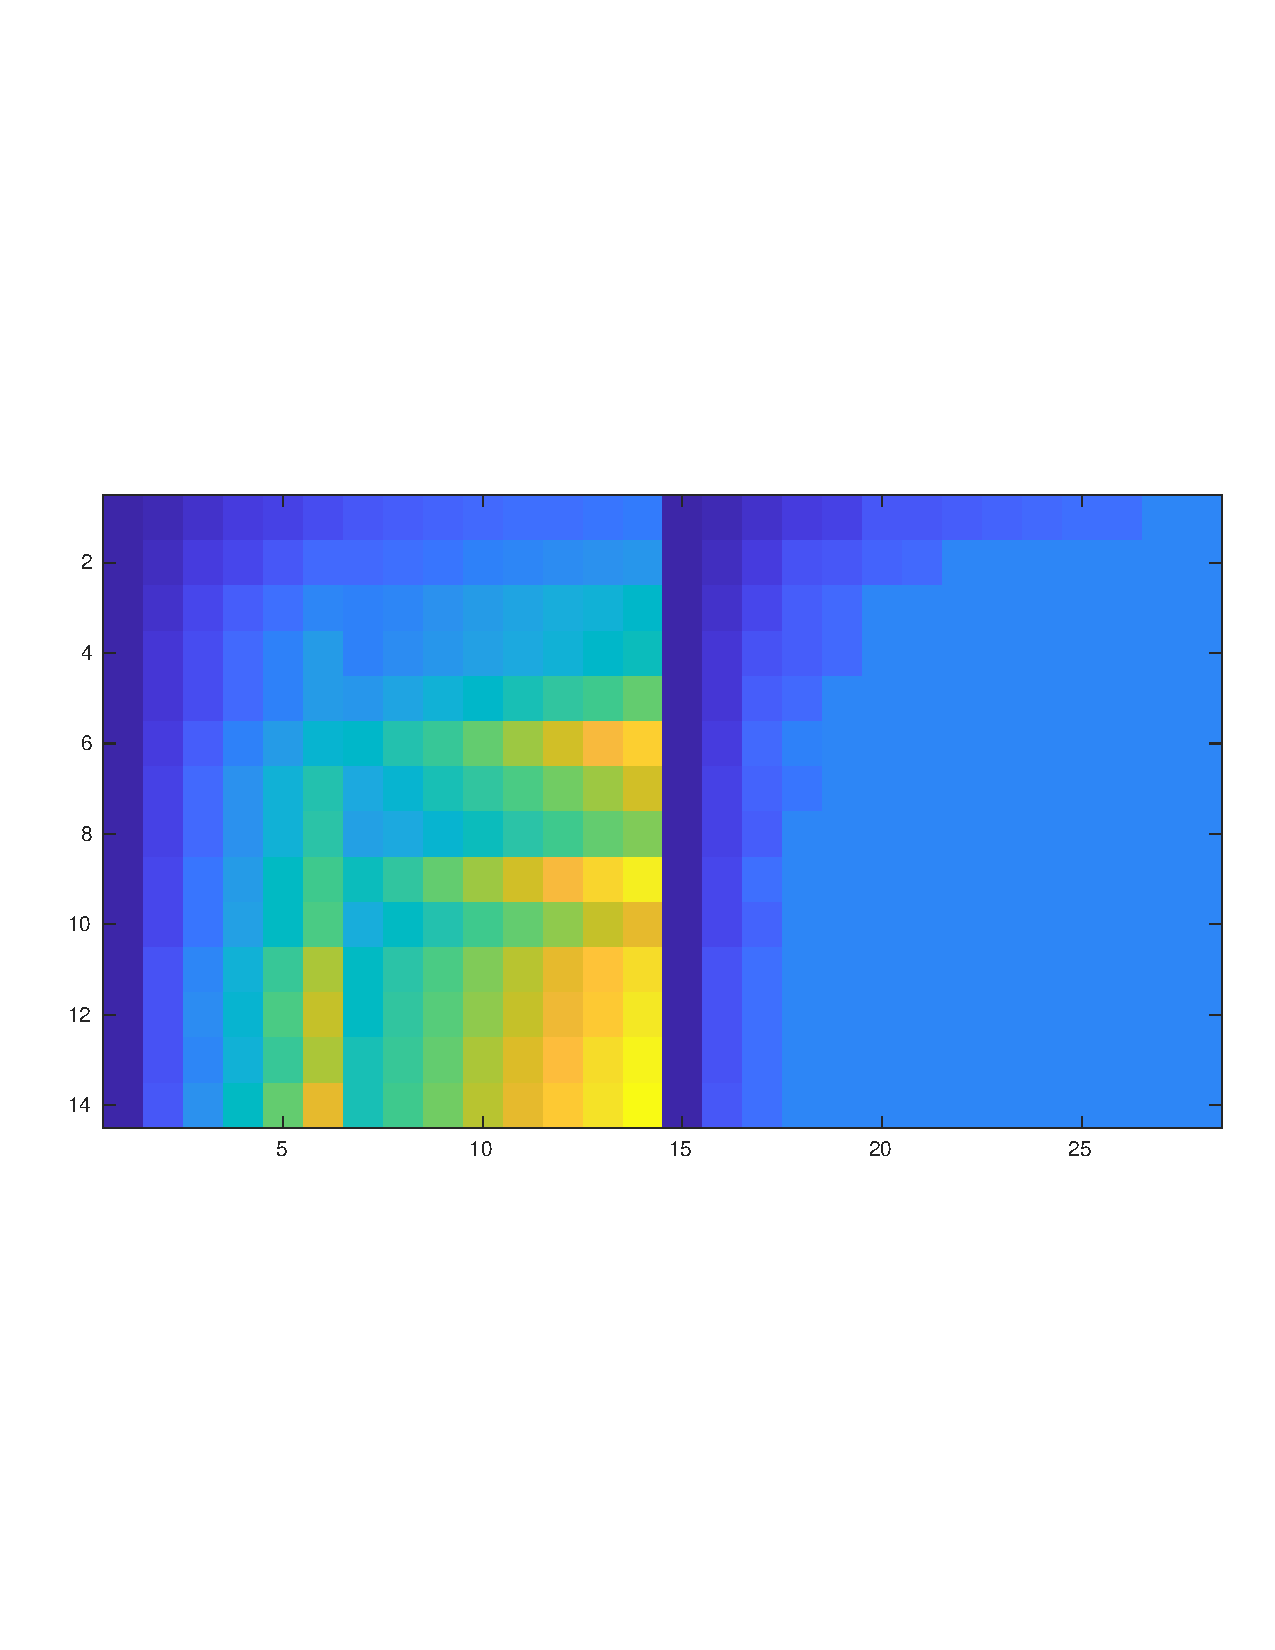
\includegraphics[width=0.99\linewidth]{images/matrix_normal.png}
\caption{Average cost (smaller the better) when sweeping the parameter $\epsilon$ (perturbation to the environment, higher implies more significant) and $c$ (the cost when caught in a storm for one time step. We assume staying in a non-storm place would have a fixed cost of 1). Each row is controlled by the same $\epsilon$ with varying $c$, and vice versa for each column. All the cost numbers are rounded to the nearest integer for the purpose of visualization. The left shows the costs from the nominal algorithm while the right from the robust algorithm. When $c=1$, the cost is the same for staying in a storm or non-storm place so both algorithms would go straight to the destination with the cost always 8. The cost of 14 (for most of the sweeps in the robust algorithm) is obtained by going along a path that avoids any possibility of getting caught in a storm (inferred from Fig.~\ref{exp_maps_normal}), and hence it is the upper bound for the cost in the robust algorithm. We can see that the robust algorithm always performs better or equally well compared to the nominal algorithm.}
\label{exp_matrix_normal}
\end{figure}

We plot the comparison of the value functions for the robust and the nominal algorithm respectively. The values are represented by a number over each state. In this experiment with grid size of 11, there is only 1 storm, indicating the total number of states is $2^1 \times 11 \times 11$. In Fig.~\ref{exp_values}, we plot the values in the form of matrices, where the left two figures are the values from the nominal algorithm, and the right two figures are the values from the robust algorithm. The difference between the top two figures (Fig.~\ref{exp_values_nostorm}) and the bottom two figures (Fig.~\ref{exp_values_storm}) is that, the values in Fig.~\ref{exp_values_nostorm} are those states with the storm off, and the values in Fig.~\ref{exp_values_storm} are those states with the storm on. 

We can observe from the values clearly that, the robust algorithm obtain a more pessimistic estimation of the cost for each locations (states). Even when there is no storm (Fig.~\ref{exp_values_nostorm}), the robust algorithm still indicates that the plane is very likely to be caught in a storm if it is inside the potential storm area. Our experimental results indicate the same as our analysis: if the initial state has no storm, the nominal algorithm would choose to go straight to the destination regardless of the huge potential the storm would occur, while the robust algorithm tends to be more conservative and takes the detour to the destination. On average of multiple roll-outs, the cost of the nominal algorithm in this case is $64.0$, and of the robust algorithm is $20.0$.

\subsubsection{Checking the cost - Storm map with a randomly generated shape}
\label{exp_normal}

The experiments in Sec.~\ref{exp_classic} provide a most friendly environment for the robust algorithm - the provided empirical transformation indicates much less probability that a storm would occur than the real environment. In this section, we compare the robust algorithm and the nominal algorithm over a randomly generated map (Fig.~\ref{exp_maps_normal}), with $4$ storms and grid size of $9$, resulting a total number of $2^4 \times 9 \times 9$ states. We conduct a more detailed evaluation of the cost and perform the analysis.

\medskip

Two factors strongly affect the behaviour of the two algorithms: the perturbation factor $\epsilon$ (which is approximately proportional to $\beta$) and the cost over the storm place $c$ (we assume the cost over the non-storm place is always 1). 

\medskip

In order to observe the behaviours over all the possible $(\epsilon, c)$ pairs, we start with the experiment to sweep both two parameters. As the cardinality of the states is significantly larger than the experiments in Sec.~\ref{exp_normal}, we skip printing the value functions and instead provides the cost over all the possible $(\epsilon, c)$ pairs. For each $(\epsilon, c)$ pair, we run the roll-outs 30 times (to sufficiently take the randomness of the weather changes into account) and put them into a 2D matrix (Fig.~\ref{exp_matrix_normal}). We refer readers to Fig.~\ref{exp_matrix_normal} for the detailed explanation. Consistent to our previous analysis, the robust algorithm performs better or equally good on almost every state compared to the nominal algorithm.


\begin{figure}
\centering
\begin{subfigure}{0.5\linewidth}
    \centering
    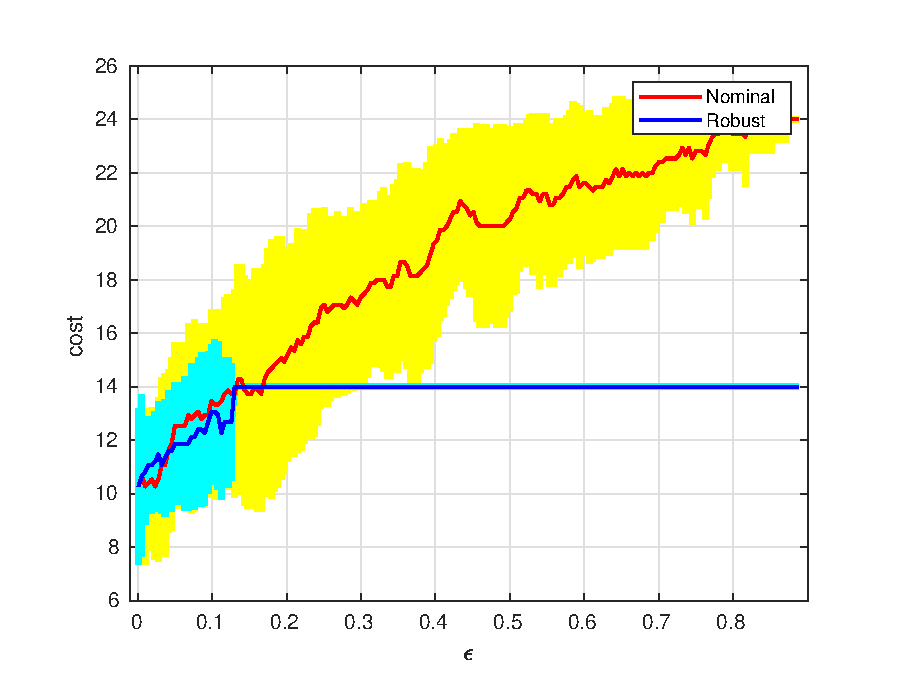
\includegraphics[width=0.9\linewidth]{images/curve_normal_epsilonSweep_new.eps}
    \caption{The average cost (vertical) and the standard deviation of the $epsilon$-sweep (horizontal). We fix $c$ to be 5.}
    \label{exp_curves_normal_epsilonSweep}
\end{subfigure}%
\begin{subfigure}{0.5\linewidth}
    \centering
    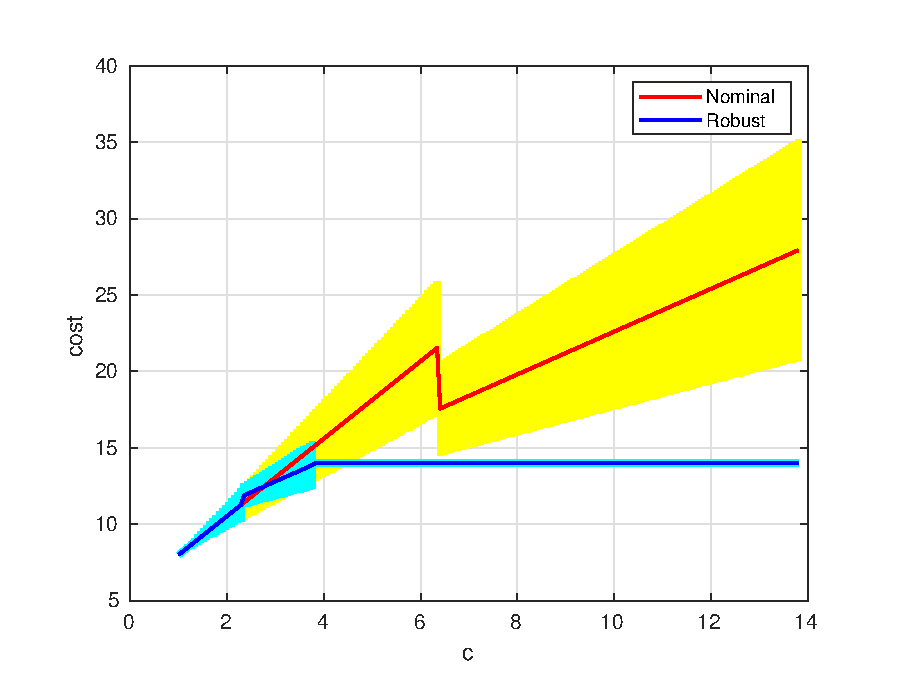
\includegraphics[width=0.9\linewidth]{images/curve_normal_costSweep_new.eps}
    \caption{The average cost (vertical) and the standard deviation of the $c$-sweep (horizontal). We fix $\epsilon$ to be 0.32.}
    \label{exp_curves_normal_costSweep}
\end{subfigure}
\caption{The average cost and the standard deviation of the sweeps.}
\label{exp_curves}
\end{figure}

To further analyze the robust algorithm in detail, we further provide two error-bar curves in Fig.~\ref{exp_curves}, with each fixing one parameter and sweeping the other. In Fig.~\ref{exp_curves_normal_epsilonSweep}, we fix $c$ to be 5 and sweep the $\epsilon$, while in Fig.~\ref{exp_curves_normal_costSweep}, we fix $\epsilon$ to be 0.32 and sweep $c$. Once again, the robust algorithm outperforms the nominal one under almost any parameter settings.

\medskip

Although in our algorithms, the robust algorithm is better under many different experimental settings, we do not claim the robust algorithm always provide us a better strategy under any case. For instance, if the true environment has higher probability of having good weather, then the overly conservative robust algorithm would instead provide us with a sub-optimal detour path, resulting in larger delays.

%%%%%%%%%%%%%%%%%%%%%%%%%%%%%%%%%%%%%%%%%%%%%%%%%%%

\section{Application: Machine Replacement Problem}

%%%%%%%%%%%%%%%%%%%%%%%%%%%%%%%%%%%%%%%%%%%%%%%%%%%

\subsection{Problem Formulation}
Machine replacement problems concerns the type of machine that deteriorates over years, and decisions need to be made over when to repair the machine. For simplicity, such problem can be modelled as a MDP process where the cost of repair is subjected to uncertainty. This formulation can be addressed by the robust type algorithms. 

\medskip

In reality, a factory may own high number of machines and they want a repair schedule that minimizes the expectation over all the machines with some probability confidence. Such formulation matches exactly with the chance constraint formulation. 

\medskip
So we investigated the performance of different formulation given two type of uncertainty set - uncertain reward and uncertain transition matrices. For the uncertain reward, we experimented the simple case that all the reward follows Gaussian distribution, so the problem can be solved via SOCP. An instance of this problem with fixed uncertainty in rewards, is shown in Fig \ref{machine_reward_map}, taken from~\cite{delage2010percentile}. 




\begin{figure}
\centering
    \includegraphics[width=0.8\linewidth]{images/mrp.pdf}

 \caption{Machine replacement problem with uncertain rewards~\cite{delage2010percentile}, each circle represents one state, the black arrow denotes the transition if the agent chooses to repair and the dotted arrow denotes the transition if the agent chooses to do nothing, each transition accompanies a uncertain reward from a Gaussian distribution.}
\label{machine_reward_map}
\end{figure}

\medskip
For the second case, the uncertain transition matrix follows the Dirichlet distribution. The robust optimization is done using the likelihood and entropy models introduced in Section 3.


%%%%%%%%%%%%%%%%%%%%%%%%%%%%%%%%%%%%%%%%%%%%%%%%%%%

\subsection{Numerical Results}
For the uncertain Gaussian reward case, the cumulative reward histogram over different algorithms are displayed in Fig \ref{machine_reward_distribution}. We ran 1000 trials for each experiment. Each experiment uses an environment with deterministic reward sampled from a random distribution. 

\begin{figure}
    \centering
    \includegraphics[width=0.8\linewidth]{images/MR-cost.png}
\caption{Cumulative cost of Chance constraint, Nominal, and robust}
\label{machine_reward_distribution}
\end{figure}

\medskip

For the uncertain transition matrix case, the cumulative cost for nominal and robust policies are shown in Fig \ref{machine_transition_plot}. It is seen that the nominal case is actually better than the robust version in our experimental settings. This is probably because the environment was more favourable for nominal and did not have sufficient perturbations, so the conservative robust policy is sub-optimal. The paper \cite{delage2010percentile} mentions that chance constraint policy once again provides the optimal policy for this problem setting.

\begin{figure}
\centering
    \includegraphics[width=0.7\linewidth]{images/mrp_trans.png}

\caption{Machine replacement problem with transitions, the figure described the problem is from~\cite{delage2010percentile}, each circle represents one state, the black arrow denotes the transition if the agent chooses to repair and the dotted arrow denotes the transition if the agent chooses to do nothing, each action has multiple possible outcomes with a probability on the line.}
\label{machine_reward_map}
\end{figure}


\begin{figure}
    \centering
    \includegraphics[width=0.4\linewidth]{machine_transition_plot.png}
\caption{Expected cost of machine replacement problem with uncertain transition matrix for nominal and robust policies}
\label{machine_transition_plot}
\end{figure}
%%%%%%%%%%%%%%%%%%%%%%%%%%%%%%%%%%%%%%%%%%%%%%%%%%%

\section{Conclusion}
We verified the expected behavior of nominal, robust and chance constrained approach to Markov Decision Processes:
\begin{itemize}
\item \textbf{Nominal strategy}: This is `blind to risk', so it incurs a high cost or low reward if the environment has large fluctuations.

\item \textbf{Robust strategy}: This is conservative, so it performs better than the nominal only when the environment has drastic variations. However, it does not use prior knowledge of the perturbation statistics but optimizes for the worst case scenario, often resulting in a sub-optimal policy.

\item \textbf{Chance constrained policy}: This is a compromise between the 2 previous strategies. i.e. it uses extra information about environment statistics to calculate a policy based on a preferred level of risk. Hence it outperforms the robust strategy when compared over multiple iterations.
\end{itemize}

%%%%%%%%%%%%%%%%%%%%%%%%%%%%%%%%%%%%%%%%%%%%%%%%%%%

\bibliographystyle{plain}
\bibliography{reference}

%%%%%%%%%%%%%%%%%%%%%%%%%%%%%%%%%%%%%%%%%%%%%%%%%%%

\end{document}
